\chapter{Gestión del proyecto.}\label{sec:gestion}

En este capítulo se describe la gestión del proyecto: ciclo de vida, planificación,
presupuesto, etc.

\section{Ciclo de vida.}

\paragraph{}Como proyecto de ingeniería el ciclo de vida podríamos dividirlo en el
esquema tradicional de:

\begin{enumerate}
  \item Comienzo de proyecto.
  \item Organización y planificación.
  \item Desarrollo.
  \item Entrega.
\end{enumerate}

\paragraph{}El comienzo del proyecto ha sido la fase más temprana en la cuál se ha
decidido el tema del proyecto, atendiendo a las necesidades o premisas iniciales. Como
recordatorio, saber que partíamos de una pequeña empresa que quería un entorno de desarrollo
integral para sus ingenieros, dicho entorno debía ser muy flexible y universal, preparado
para cumplir con los requisitos típicos de las \glsplural{startup}.

\paragraph{}La organización y planificación ha consistido, como su propio nombre indica,
en dividir todas las fases del desarrollo y entrega dentro del tiempo marcado, teniendo
en cuenta la disponibilidad personal. Para cada fase del desarrollo se ha fijado una
fecha límite, como si fuese una entrega parcial.

\paragraph{}El desarrollo del proyecto ha consistido en toda la creación de ingeniería,
desde el diseño y especificación, hasta la entrega. En la siguiente sección \ref{sec:planificacion}
se detalla más las subfases de esta etapa.

\paragraph{}La fase de entrega ha consistido en la comprobación y evaluación de los
objetivos planteados, en la redacción de esta memoria y en la cosideración de ampliaciones
futuras.

\section{Planificación.}\label{sec:planificacion}

\paragraph{}Debido a que el proyecto es unipersonal y no se ha podido simultanear tareas,
se ha desarrollado un modelo en cascada. En cualquier caso, por costumbre del autor,
se va a tratar la planificación en terminos ágiles,
específicamente de la metodología de SCRUM.

\begin{figure}[H]
    \centering
    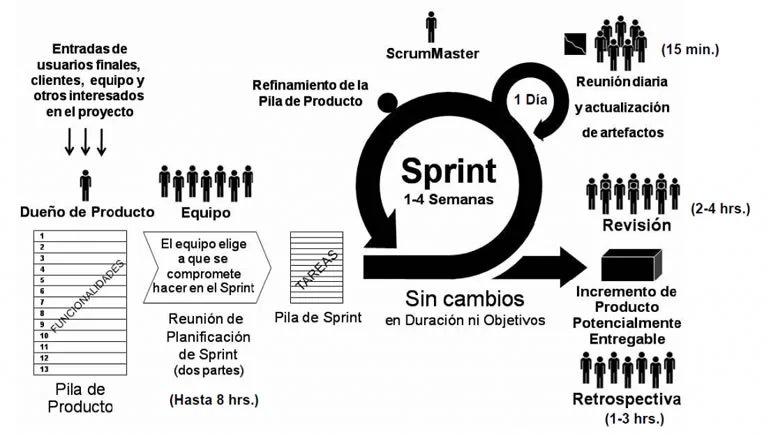
\includegraphics[width=0.85\textwidth]{imgs/scrum}
    \caption{Figura de una metodología SCRUM paradigmática}
    \label{fig:scrum}
\end{figure}

\paragraph{}Así, la planificación ha constado de cuatro ``sprints'' de cuatro cascadas
de aproximadamente una semana de duración cada uno.

\begin{figure}[H]
    \centering
    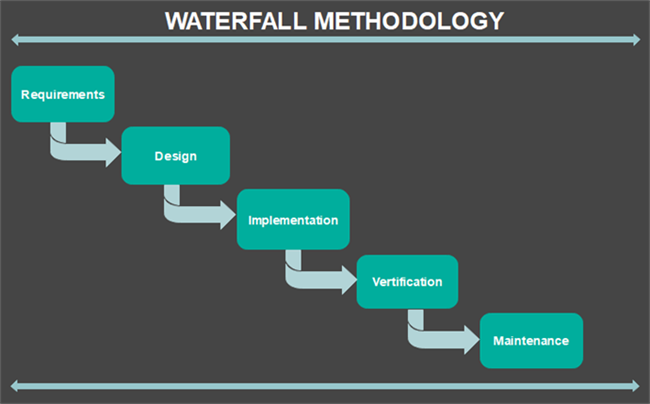
\includegraphics[width=0.85\textwidth]{imgs/waterfall}
    \caption{Figura de una metodología en cascada o \emph{waterfall}}
    \label{fig:waterfall}
\end{figure}

\subsection{Sprint 1: Entorno de desarrollo general.}

\paragraph{}Esta fase ha sido la primera, ya que ha consistido en el aprendizaje previo
de las tecnologías que han sido necesarias aplicar, probarlas por separado y comprobar
la viabiliad técnica de las especificaciones.

\subsection{Sprint 2: Aplicación Flutter.}

\paragraph{}El segundo sprint fue realizar la aplicación Flutter, se ha hecho así, ya
que Yocto trabaja recolectando fuentes de programas y compilándolos, entonces se
necesitaba tener primero una aplicación. Además, Flutter, por
diseño, compila las aplicaciones en cualquier plataforma por lo que se podía desarrollar
la aplicación, verla y probarla sin tener el sistema operativo final, ni conocer la
arquitectura hardware definitiva. Al final de este sprint, se tenía una aplicación plenamente
operativa para cualquier plataforma.

\subsection{Sprint 3: Yocto.}

\paragraph{}Una vez que se tuvo la aplicación Flutter desarrollada, el siguiente paso
lógico para tener listo el prototipo, era tener un sistema corriendo en el hardware.
Una vez se instaló el sistema totalmente genérico, hubo que integrarle la aplicación y realizar
las personalizaciones pertinentes.

\subsection{Sprint 4: Universalización y coherencia entre entornos.}

\paragraph{}Con el prototipo funcionando, se podría considerar que todo el entorno de
desarrollo había sido validado, pero el esfuerzo de este proyecto ha sido siempre que
el entorno de desarrollo fuera \emph{ad-hoc} a las necesidades, que estuviese preparado
para funcionar de la manera más sencilla y flexible posible. Este último sprint fue el
más complicado y posiblemente el que más atención requirió.

\section{Presupuesto.}

\subsection{Personal.}

\paragraph{} En este caso, el proyecto ha sido llevado a cabo por un sólo desarrollador.
Incluyendo la fase de planificación, diseño y desarrollo, la dedidación en horas ha sido
aproximadamente de un mes a media jornada (6 horas), además debemos tener en cuenta el
nivel de conocimientos trasnversales propios de un ingeniero senior.


\begin{table}[hbt]
	\label{t:recursoshumanos}
	\centering
	\begin{tabular}{|c|c|c|c|c|}
		\hline
        \textbf{Días trabajados} & \textbf{Horas al día} & \textbf{Total} & Precio [\euro/hora] & \textbf{Total} \\
		\hline
		22 & 6 & 132 & 15 & 1980 \\
		\hline
	\end{tabular}
	\caption{Desglose de horas dedicadas.}
\end{table}

\subsection{Material.}

\paragraph{}Los materiales utilizados son una Raspberry Pi rev.3B+, una tarjeta microSD
de 16 Gb, un cable de alimentación, una fuente alimentación, una pantalla LCD 5" táctil,
y una carcasa impresa en 3D.


\begin{table}[hbt]
	\label{t:materialescostes}
	\centering
	\begin{tabular}{|c|c|c|c|}
		\hline
		\textbf{Producto} & \textbf{Coste unidad [\euro]} & \textbf{Cantidad} & \textbf{Subtotal [\euro]} \\
		\hline
		Rbpi rev.3B+ & 37 & 1 & 37 \\
		\hline
		microSD & 10 & 1 & 10 \\
		\hline
        Alimentación & 15 & 1 & 15 \\
		\hline
        Pantalla LCD 5" & 20 & 1 & 20 \\
		\hline
        Carcasa 3D & 5 & 1 & 5 \\
		\hline
		\textbf{Total} & & & 87 \\
		\hline
	\end{tabular}
    \caption{Desglose de presupuesto de materiales.}
\end{table}

\subsection{Otros costes.}

\paragraph{}Dentro de esta sección podremos considerar, por ejemplo:

\begin{itemize}
    \item Licencias de software.
    \item Suscripciones a servicios.
    \item Factura de la luz.
    \item Gastos de papelería.
    \item Etcétera.
\end{itemize}

\paragraph{}Sin entrar en demasiado detalle podemos estimar una cantidad
para el total de conceptos descritos anteriormente de 30\euro.

\subsection{Resumen de costes.}

\paragraph{}Teniendo en cuenta los costes desglosados en los apartados anteriores, el
presupuesto del proyecto queda de la siguiente manera:

\begin{table}[hbt]
	\label{t:resumencostes}
	\centering
	\begin{tabular}{|c|c|}
		\hline
		\textbf{Concepto} & \textbf{Gasto [\euro]} \\
		\hline
		Personal & 1980 \\
		\hline
		Material & 87 \\
		\hline
		Otros & 30 \\
		\hline
		\textbf{Total} & 2097 \\
		\hline
	\end{tabular}
    \caption{Resumen del presupuesto del proyecto.}
\end{table}

\paragraph{}Se puede considerar un proyecto de ingeniería barato ya que requiere de
muy pocos recursos y materiales y utiliza software de código abierto. Como suele ser
habitual en estos casos, el recurso más límitado y valioso son los recursos humanos.
Por eso, en el ámbito de las \glsplural{startup} es fundamental encontrar a gente
que tenga mucho que aportar y dar la oportunidad a becarios con mucha energía y ganas
de aprender.

\paragraph{}El presupuesto refleja el proyecto en un estado de \gls{MVP}. Es decir,
que es el coste de producir pocas unidades de prototipos funcionales que puedes mostrar
a \glsplural{early bird}. Y en base al feedback recogido, poder seguir buscando inversores,
mejorando la ingeniería del proyecto y llevando el producto a fase de producción.


%las referencias a artículos se ponen con \cite,
%las referencias a glosario \gls,
%y las referencias a ecuaciones \eqref
%las referencias a imgenes, tablas o figuras o secciones
% se ponen con \ref (sólo número) o con \hyperref[sec:X]{text}
